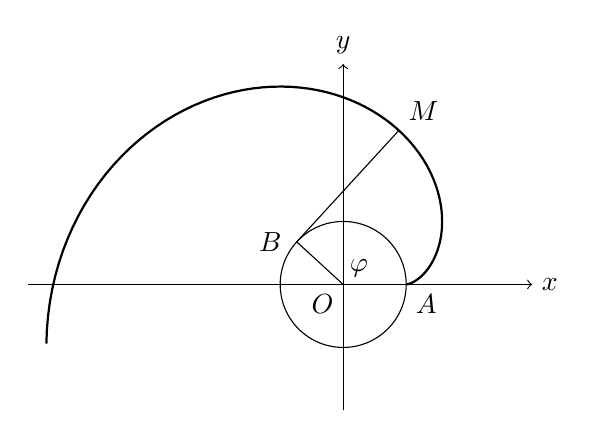
\begin{tikzpicture}[scale=0.8] % 将 scale 从 1.5 缩小到 1.0，整体图形变小
    % 1. 绘制坐标轴
    \draw[->] (-5,0) -- (3,0) node[right] {$x$};
    \draw[->] (0,-2) -- (0,3.5) node[above] {$y$};
    \node[below left] at (0,0) {$O$};

    % 2. 绘制圆与 A 点
    \draw (0,0) circle (1);
    \node[below right] at (1,0) {$A$};

    % 3. 绘制渐开线
    % 渐开线参数方程: x = r(cos t + t sin t), y = r(sin t - t cos t)
    \draw[thick, domain=0:4.7, samples=100] 
        plot ( {cos(\x r) + \x*sin(\x r)}, {sin(\x r) - \x*cos(\x r)} );

    % 4. 定义 B 和 M 的坐标 (选取 phi=2.0 rad，此时 M 点的横坐标约为 1.4，在视觉上 M 点在第一象限靠右，更符合你新给出的参考图位置)
    \pgfmathsetmacro{\phi}{2.4}
    \coordinate (B) at ({cos(\phi r)}, {sin(\phi r)});
    \coordinate (M) at ({cos(\phi r) + \phi*sin(\phi r)}, {sin(\phi r) - \phi*cos(\phi r)});
    \coordinate (O) at (0,0);

    % 5. 绘制内部连线
    \draw (O) -- (B);
    \draw (B) -- (M);

    % 6. 标注标签与角度
    \node[left, xshift=-2pt] at (B) {$B$};
    \node[above right] at (M) {$M$};
    
    % 绘制角度 \varphi
    \node at (0.25, 0.25) {$\varphi$};
\end{tikzpicture}